\documentclass{sig-alternate}
\usepackage{times}
\usepackage{amssymb,amsmath}
\usepackage{cleveref}
\usepackage{algorithm}
\usepackage{times}
\usepackage{color}
\usepackage{url}
\usepackage{subfigure}
\usepackage{xspace}
\usepackage[noend]{algorithmic}
\usepackage{enumerate}
\usepackage{multirow}
\usepackage{balance} 
\usepackage{epstopdf}
\usepackage{graphicx}

\newcommand{\model}{{{\sf SourceNote}}\xspace}
\newtheorem{definition}{Definition}
\newtheorem{example}{Example}
\newtheorem{theorem}{Theorem}
\newtheorem{problem}{Problem}
\newtheorem{reduction}{Reduction}


\begin{document}

%\title{Assessing the Quality of Data and Finding Invaluable Sources}
\title{Finding Quality in Volume: The Challenge of Discovering Valuable Sources for Integration}
%\title{SourceNote: Discovering Invaluable Data Sources in Volume}

\numberofauthors{5} 

\author{
% 1st. author
\alignauthor
Theodoros Rekatsinas\\
       \affaddr{University of Maryland}\\
       \email{thodrek@cs.umd.edu}
% 2nd. author
\alignauthor
Amol Deshpande\\
       \affaddr{University of Maryland}\\
       \email{amol@cs.umd.edu}
% 3rd. author
\alignauthor
Xin Luna Dong\\
       \affaddr{Google Inc.}\\
       \email{lunadong@google.com}
 \and
% 4th. author
\alignauthor
Lise Getoor\\
       \affaddr{UC, Santa Cruz}\\
       \email{getoor@soe.ucsc.edu}
 % 5th. author
\alignauthor
Divesh Srivastava\\
       \affaddr{AT\&T Labs Research}\\
       \email{divesh@research.att.com}
}    

\maketitle
\begin{abstract}
Data is becoming a commodity of tremendous value for many applications, leading to a rapid increase in the number of open access data sources and services, such as cloud-based data markets and data portals, that facilitate the collection, publishing and trading of data. Data sources are typically heterogeneous in their content, the quality of data they provide and the fees they may require for accessing their entries. However, when the number of data sources is large, humans have a limited capability of reasoning about the actual quality of sources the trade-off between the benefits and costs of acquiring and integrating sources. Given the sheer number of available data sources, analysts must (1) identify sources that are relevant to their integration task, (2) discover sources that potentially satisfy the quality and budget requirements of their applications with few effective clues about the quality of the sources, (3) repeatedly invest many man-hours in assessing the eventual usefulness of data sources by manually investigating their content or integrating subsets of them and evaluating the actual benefit of the integration result for their application. In this paper we explore the problems of appraising the quality of data sources and identifying the most beneficial sources for diverse integration tasks. We introduce our vision for a new data source management system that automatically assesses the quality of data sources based on a collection of rigorous data quality metrics and enables the automated discovery of valuable sources for user specified integration tasks. We argue that the proposed system can dramatically ease the {\em Discover-Appraise-Evaluate} interaction loop that many analysts follow today to discover beneficial sources for their tasks. 
\end{abstract}

% A category with the (minimum) three required fields
%\category{H.4}{Information Systems Applications}{Miscellaneous}
%A category including the fourth, optional field follows...
%\category{D.2.8}{Software Engineering}{Metrics}[complexity measures, performance measures]

%\terms{Theory}

%\keywords{ACM proceedings, \LaTeX, text tagging} % NOT required for Proceedings

\section{Introduction}
In the last few years, the number of data sources available for integration and analysis has risen because of the ease of publishing data on the Web, the proliferation of services that facilitate the collection and sharing of data (e.g., Google Fusion Tables), and  the adoption of open data access policies both in science and government. This deluge of data has enabled small and medium enterprises as well as data enthusiasts to increasingly acquire and analyze data from multiple data sources. 

However, the sheer number of available data sources makes it challenging for a user to identify sources that are truly beneficial to her integration or analysis task. First, many sources provide erroneous or stale data entries that can be detrimental to the quality of integration~\cite{Dong_vldb:2009, li:2012} or provide  duplicate and redundant data making hard to identify the unique information a source is providing~\cite{bronzi:2013, li:2012}. Second, sources exhibit significant heterogeneity in representation of stored data (e.g., the schema they follow), making it challenging for a user to discover all relevant sources for her integration task~\cite{dassarma:2012}. Finally, acquiring and integrating data comes with a monetary and computational cost, and hence, integrating every available source may not be worthwhile or even feasible due to budget constraints. These challenges give rise to the natural questions of (i) how can one specify the value of data in a rigorous fashion and (ii) how can one identify the most beneficial data sources for arbitrary integration tasks. 

In recent work~\cite{dong:vldb13, rekatsinas:2014} we showed that given a fixed data domain, the benefit of integration can be specified using rigorous quality metrics such as {\em coverage}, {\em accuracy} and {\em freshness}. We also introduced the paradigm of {\em source selection} to reason about the benefits and costs of acquiring and integrating data. Yet our proposed techniques focus on pre-defined integration tasks and do not provide support for a diverse set of users to specify their integration task. Moreover, our approach requires that a user knows exactly which quality metric is of importance to her or what her desired trade-off between multiple metrics is. This last requirement is rather unrealistic as users rarely know what is the right trade-off between different quality metrics. 

In this paper we introduce our vision for a {\em source management system} that will enable users to specify heterogeneous integration tasks as keyword queries and allow them to interactively discover the most important sources for their specified task. Given an extensive collection of rigorous data quality metrics, we envision a system that automatically discovers the quality of different data sources and extends our idea of source selection to enable discovery and exploration of data sources. A key characteristic of the proposed system is to facilitate users understand which quality metrics are important for their integration task and enable them to discover sources whose integration result will maximize the desired metrics under any specified budget constraints. 

The remainder of the paper is organized as follows. In \Cref{sec:discovery} we discuss the key requirements and challenges in building a data source management system, including, defining and computing multiple quality metrics that characterize the content of sources, supporting diverse integration tasks expressed as keyword queries,  and enabling the interactive exploration of data sources. Then, \Cref{sec:overview} presents and overview of our proposed system, introduces the different modules of the system and proposed  techniques for addressing the aforementioned challenges. Finally, \Cref{sec:related} discusses related work and \Cref{sec:conclusion} concludes the paper. 

\section{Discovering Valuable Sources}
\label{sec:discovery}
In this section we describe two tasks that require integrating data from multiple sources. Our goal is to identify common characteristics across diverse tasks and building upon these introduce the main operations that a source management system should be able to support for discovering valuable sources. Finally we describe the challenges in each of these operations.

\subsection{Motivating Examples}
\label{sec:example}
Our goal is to demonstrate how data from multiple sources can be combined to perform diverse tasks and what are the main characteristics that one can use to fully specify diverse integration tasks. The first task we consider corresponds to combining data from multiple news papers to validate a new theory in political scienses, while the second one corresponds to a company converting social media activity into early signals to spot emerging trends for Fortune 500 companies, news organizations and financial institutions. 

We consider the Global Database of Events, Languages and Tone (GDELT)~\cite{leetaru:2013} where news articles from thousands of news domains (sources) are aggregated in a single repository. The articles are analyzed and events, defined as pairwise interactions between actors, are extracted from them. Actors typically correspond to well-known organizations, including countries or international organizations. The extracted events are quite diverse ranging from economic agreements between companies to violent acts between parties and are associated with certain locations, actors (corresponding to organizations), and a description containing the political views of the actors and a characterization of the event. Such a repository can be used for diverse analytics tasks. We focus on a scenario where analysts integrate events mentioned in a diverse set of news media sources and analyze them collectively to detect patterns and evaluate new theories. In particular, we focus on the work by Schutte et al.~\cite{schutte:2014}. In this work, the authors focus on finding causal relationships in spatiotemporal event data and use data from GDELT to build test cases for validating their theory. In particular, they are interested in examining how the civilian assistance to US forces changed in response to indiscriminate insurgent violence in Iraq. They focus on a specific time-window from 2003 to 2010, consider events in specific locations in Iraq and consider actors corresponding to specific ethnic groups in Iraq.

Next, we consider the company TrendSpottr~\cite{trendspottr} and its partnership with Datasift~\cite{datasift}. Datasift is a company that extracts social media data from multiple sources, including Twitter, Facebook, Blogs etc., and offers a common API for accessing dozens of different data sources in real-time. TrendSpottr analyzes real-time data streams such as Twitter and Facebook to spot emerging trends at their earliest acceleration point. They require access to historical data, demographic information and geo location information as all of this data is important to the predictive model used by the company. Typical tasks supported by TrendSporttr are viral news discovery corresponding to different locations and specific organizations, brand and reputation monitoring, ranging from company acquisitions to sports,  market predictions and many others. 

In both scenarios, we see that specifying an integration task involves providing information about its {\em location}, a set of exact instances or types of {\em organizations} or {\em people} involved in it and a {\em time window} associated with the task (this can be either a real-time task or a historical task over a past time-window). Moreover, it is easy to see that different types of data quality are implicitly relevant to each of the aforementioned tasks. For example, {\em completeness} is important for the first task but timeless is not crucial as delayed mentions of events will not affect the quality of the analysis. On the other hand, {\em timeliness} is very important in the second application. Analyzing sources that exhibit significant delays beats the purpose of the application which is early detection of trends. 

\subsection{Key Operations}
\label{sec:operations}
Building upon the previous examples, we present the main operations that a source management system should support for discovering valuable sources.  First, we consider the input to such a system. We argue that the system should ask a user to specify a desired integration task providing the following information: (i) a keyword description of the integration task corresponding to a collection of mentions to either specific objects or types (concepts) of locations, organizations and people, (ii) a selection of relevant data quality metrics from a list of supported metrics, and (iii) a desired budget characterizing the amount of money the user can afford for acquiring data. Given these specifications as input  a source management system should perform the following operations:
\begin{enumerate}
\item {\bf Discover.} Given the keyword description of the integration task the system should automatically determine which sources are relevant to the task by mapping the content of the task description to the content of sources.
\item {\bf Appraise.} Once the system has discovered a set of relevant sources to the user's integration task it should detect automatically subsets of sources that if integrated together the quality of integrated data will be maximized with respect to the specified quality metrics and the imposed budget constraints. The system should identify multiple solutions that correspond to different trade-offs among the quality metrics specified by the user in a try to diversify the solutions presented to the user in the last phase. Exploring different quality metric trade-offs is necessary for the user to understand what are the exact quality characteristics required for her task.
\item {\bf Evaluate.} The solutions discovered in the previous phase should be presented to the user together with a concise description of their quality characteristics as well as a description of the data sources included in each of them. Moreover, the user should be able to explore the neighborhood of a solution by removing sources or examining solutions with similar characteristics that contain different sources.
\end{enumerate}

\subsection{Challenges}
Next, we discuss the main challenges in each of the operations presented above. 
\subsubsection{Diverse Integration Tasks}
\label{sec:diverse}
The first challenge is supporting integration tasks over heterogeneous data domains. As illustrated in the previous examples, the different concepts or entities associated with an integration task can vary significantly. Moreover, the data from the sources can be both structured and unstructured. Therefore, a data source management system should be able to reason about the semantic content of different types of data ranging from tables to free-text. Moreover, the system should be able to analyze the content of the user-provided task description without requiring a specific schema or considering only a pre-specified set of terms. Once the content is analyzed it should be semantically matched to the content of the available sources included in the system. To fulfill these requirements one should be able to support scalable search over different types of data (e.g., structured and unstructured) while following an open-domain assumption and not restricting user queries to a pre-specified vocabulary.

\subsubsection{Data Source Quality} 
\label{sec:quality}
The second challenge is defining the quality of data and being able to assess the quality of different sources in an automated way. Traditionally, the quality of data sources had been measured using the amount of erroneous information provided by the source. However, as discussed earlier there are multiple quality metrics that might be of interest to a user. 

Given an integration task $\mathcal{I}$ let its data universe $\mathcal{U}(I)$ to be the set of all objects that are relevant to task $\mathcal{I}$. Notice, that $\mathcal{U}(I)$ is not fully known but only partial information is available for this universe via the data sources. We assume that each object $r \in \mathcal{U}(I)$ has a set of attribute values denoted by $r.A$. For example these attributes can correspond to a location or a type or instance of an organization as described in the previous examples. Moreover, we assume that either the objects in $\mathcal{U}(I)$ or their values may change over time. Given a set of sources $S$ relevant to task $I$ and an integration model $F$ we have that $F(S) \subseteq \mathcal{U}(I)$, where $F(S)$ denotes the set of objects extracted after integrating all sources in $S$. Using this notation we define the following metrics:

\vspace{5pt}\noindent\textbf{Coverage.} The coverage of $S$ with respect to $\mathcal{U}(I)$ can be defined as the probability that an object chosen from $\mathcal{U}(I)$ uniformly at random will be present in $F(S)$. Notice that we do not require that the attributes of the object $r.A$ are correct.

\vspace{5pt}\noindent\textbf{Accuracy.} The accuracy of $S$ with respect to $\mathcal{U}(I)$ can be defined as the probability that an object chosen from $F(S)$ uniformly at random is correct with respect to $\mathcal{U}(I)$. The latter means that the object must be present in $\mathcal{U}(I)$ and all its attributes should have the correct values capturing errors due to both noisy and stale data.

\vspace{5pt}\noindent\textbf{Timeliness.} The timeliness of $S$ with respect to $\mathcal{U}(I)$ can be defined as the cumulative probability distribution of a change in the objects of $\mathcal{U}(I)$ being reflected in $F(S)$ with a delay of at most $t$ time units. Notice that this last quality metric does not correspond to a single number but an entire distribution characterizing the delays the source exhibits.

\vspace{5pt}Notice that all definitions presented above, compare the content of a source or a set of sources with the data universe corresponding to an integration task. However, the actual content of the universe is unknown and only partial information is available via content samples from the sources. Given this, the main challenge becomes combining the available source samples to extract a sufficient view of the data universe. Another challenge is that one should be able to compute the aforementioned quality metrics efficiently for any set of sources. Computing the quality of any possible set of sources in advance is obviously prohibitive. However, for certain cases~\cite{dong:vldb13,rekatsinas:2014}, one can estimate the overall quality for any set of sources by building offline quality profiles for each individual source and then combining those during source selection to estimate the overall quality for an arbitrary set of sources. The high-level intuition behind this approach is that each of the aforementioned quality metrics is associated with a random variable following a specific probability distribution (i.e., a Bernoulli distribution for coverage and accuracy and an empirical distribution for timeliness). If the sources are assumed to be independent the corresponding random variables are also independent, and hence, the probabilities corresponding to the quality of a set of sources can be computed efficiently using the decomposable disjunction formula. For example, the overall coverage for a set of sources $S_1$ and $S_2$ with individual coverages $C(S_1) = 0.6$ and $C(S_2) = 0.7$ corresponds to the probability that an item from $\mathcal{U}(I)$ is either covered by $S_1$ or covered by $S_2$ and is $C(S_1,S_2) = 1 - (1-0.6)(1-0.7) = 0.88$.


In reality, however, sources are far from independent~\cite{berti-equille:sailing, dong:2009}, as they exhibit overlaps, copying relationships and/or may contradict each other. These relationships make the quality random variables for each source dependent. Estimating the aforementioned quality metrics under the presence of dependencies imposes a major challenge as: (i) it  requires extracting the source dependencies from available source samples and (ii) devising efficient techniques for computing the probability of the overall quality random variables during query evaluation. In fact, the latter often corresponds to performing probabilistic inference over a joint distribution formed by the quality random variables corresponding to the desired set of sources.

\subsubsection{Interactive Evaluation}
\label{sec:eval}
As mentioned above, users should be able to specify a certain budget for their integration task. This can be either a monetary budget, limiting the amount of data that can be acquired, or a budget on the number of sources that a source selection solution should contain. The latter is particularly useful when a user wants to verify the content of sources manually. While specifying a constraint on the integration budget is natural to users, specifying a constraint on the data quality with respect to the aforementioned metrics is rather intricate due to the interdependencies between the different metrics and we expect that not even expert users know the exact data quality requirements of a task. Consider for example a political scientist analyzing news papers articles to forecast interesting events. Imposing a constraint on using only data sources that have exhibited zero delay with respect to certain events may reduce the accuracy of the integration result. Moreover, users may not know what is the feasible level of quality given their budget and what are the trade-off between solutions that focus on maximizing the different quality metrics in isolation. For example, selecting sources optimizing for accuracy may lead to an integration result of low coverage.  

So a major challenge for a source management system is to guide the user through the different source selection solutions that satisfy the user's budget and help her understand the trade-off between the integration quality achieved by different solutions. We argue that this is feasible only through an interactive process where the user will be able to explore the feasible solution space following suggestions of the source management system. This will enable users to understand the interdependencies between the different quality metrics with respect to their integration task and identify the particular solution that suits their application. The latter raises the following challenges: (i) how can a user explore the solution space efficiently, (ii) how can a source management system present the quality profile for a set of sources in a concise and meaningful way, and (iii) what are the right hints that the system should present to the user to facilitate the exploration of the solution space. 

\section{System Overview}
\label{sec:overview}
In this section we propose a preliminary design that aims to address the challenges specified in the previous section. An overview of the proposed architecture for a data source management system is show in \Cref{fig:system}. The system is composed by (i) a data extractor module, responsible for collecting the raw data from different sources, (ii) a source analysis engine that is responsible of analyzing the content of sources, evaluating their quality with respect to the quality metrics introduced in the previous section and creating an index describing both the content and containing a quality profile for each source, and (iii) a query engine that given a user query (i.e., a description of the desired integration task), is responsible of identifying the data domain corresponding to the query, the relevant sources, find the most valuable sources based on source selection and present the results to the user while enabling interactive exploration. Next, we focus on the source analysis engine and the query engine and discuss how these two components address the challenges and requirements presented above. We omit the first module of extracting data from different sources as it does not entail any technical challenges.

\begin{figure}
	\begin{center}
	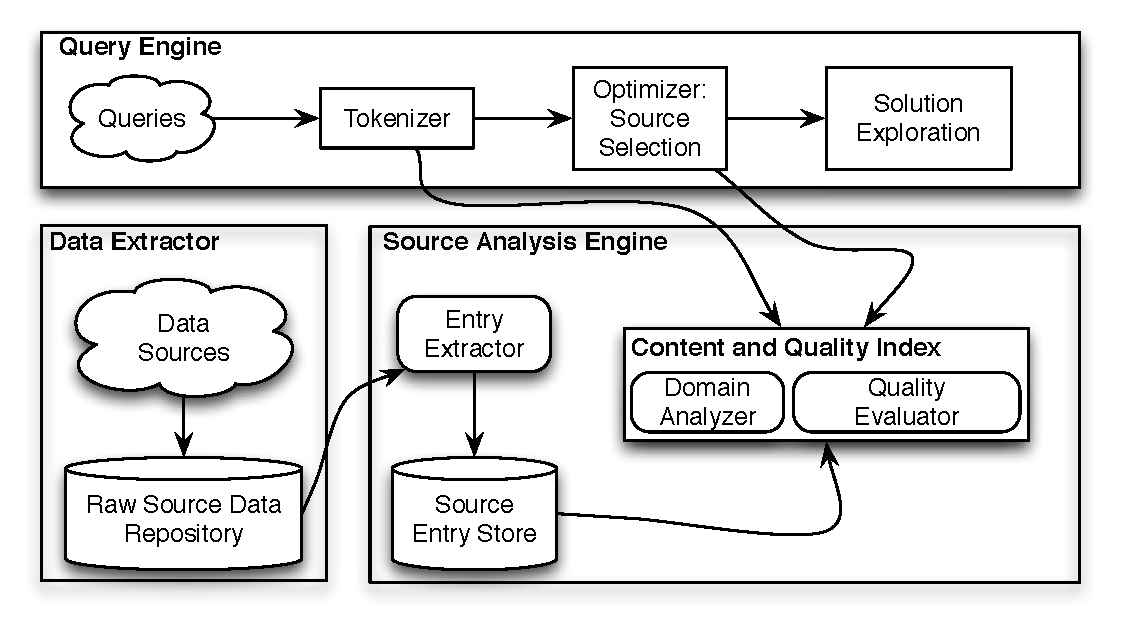
\includegraphics[clip,scale=0.5]{fig/system.eps}
	\caption{Source Management System Architecture.}
	\label{fig:system}
	\end{center}
\end{figure}


\subsection{Source Analysis Module}
A data source management system should be able to support sources covering completely heterogeneous data universes. For example, it should be able to analyze the content of a structured Web table providing financial data and the unstructured content of news articles extracted from a news paper. This is necessary for diverse integration tasks as described in \Cref{sec:diverse}. 

We propose using a {\em knowledge graph}, i.e., a {\em knowledge base} organized as a graph (e.g., Google Knowledge Graph), as a global relaxed schema for describing arbitrary data universes. A knowledge base acts as an information repository that provides a means for information to be collected, organized, shared, searched, and utilized. A knowledge base can be viewed as a collection of {\em facts} that describe information about entities and their properties, and {\em concepts} that describe information about entity types and their properties. Both facts and concepts can be represented as nodes of the knowledge graph. Given a knowledge graph, a data universe (e.g., ``Sports in the USA") can be described as a collection of concepts and/or entities. To reason about the different data universes the available sources cover and the source quality we propose augmenting the knowledge graph with a {\em correspondence graph}.

\begin{figure}
	\begin{center}
	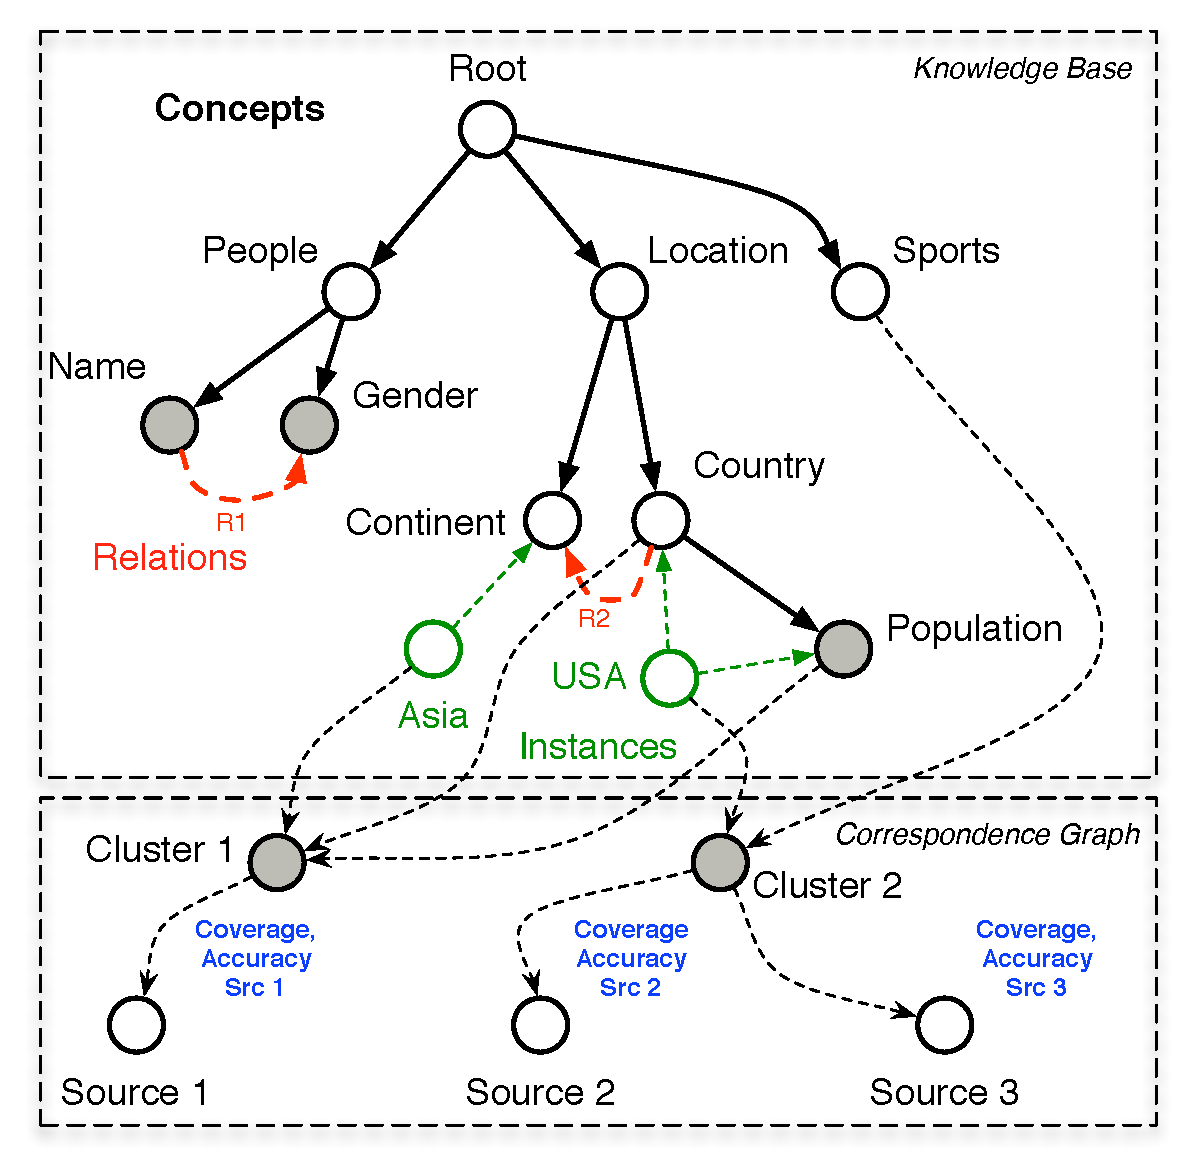
\includegraphics[clip,scale=0.4]{fig/kgcg}
	\caption{An example of a knowledge graph and a correspondence graph with a universe node corresponding to the population of countries in Asia.}
	\label{fig:kgcg}
	\end{center}
	\vspace{-20pt}
\end{figure}

Specifically, the correspondence graph contains data sources as nodes (referred to as {\em source nodes}), a set of nodes corresponding to clusters of concepts and/or entities as dictated by the available sources (referred to as {\em universe nodes}), and connects each source node with the universe node corresponding to the concepts and facts covered by that source. The universe nodes are also connected with the corresponding concepts and entities.  Each edge from a source to a universe node is annotated with a quality profile of that source for that specific data universe, and each universe node is associated with local information about the dependencies of the data sources that are connected to it. An example of a knowledge graph and a correspondence graph is shown in \Cref{fig:kgcg}. Next, we describe a preliminary approach for constructing the correspondence graph. We propose a two step approach where we first learn the universe nodes for a set of data sources and then compute the quality profiles and data source dependencies for each universe node. 

The universe nodes in the correspondence graph correspond to a clustering of the content of the available data sources. Furthermore, each of these nodes is associated with a collection of concepts and/or instances of the knowledge graph. The following approach can be used to construct these nodes. Each source can be viewed as a {\em collection of entries}, where each entry is a {\em conjunction} over concepts and/or instances. To obtain this representation, we must annotate the content of each source with concept and instance labels from the knowledge graph. Several techniques have been proposed for obtaining these annotations~\cite{spotlight,limaye:2010}. Once the content of sources is represented as a collection of concept and instance conjunctions, one can use a {\em mixed membership model}~\cite{blei:2003} to describe how the content of sources is generated considering the universe nodes. Each source is modeled as a mixture over the universe nodes. The universe nodes are shared across all sources but the mixture proportions vary from source to source (they can also be zero). Each universe node describes a distribution over concepts or events. We plan on building upon recent work on sparsity inducing non-parametric latent variable learning techniques~\cite{elidan:2005, sdm:2013}. Sparsity is necessary as each universe node should contain only a small number of concepts and instances. 

After learning the universe nodes in the correspondence graph we can collectively analyze the relevant content of all sources corresponding to each node in order to extract a quality profile for each source. In particular, we propose following an approach similar to Rekatsinas et al.~\cite{rekatsinas:2014} where samples from all the sources are integrated into a single dataset corresponding to the content of the data universe and then each individual sample is compared with the integrated data to extract the source quality profile. 

Apart from the individual source quality profiles we also need to learn the quality dependencies across different sources. Recall that the quality metrics presented in \Cref{sec:quality} 
can be expressed as probabilities corresponding to a distribution associated with source-quality random variables. In fact when sources are dependent these random variables are dependent, and hence, these dependencies need to be extracted from the available source samples.  We conjecture that these dependencies can be represented using a {\em factor graph}, i.e., a particular type of graphical model that enables efficient computation of marginal distributions, over the source random variables. We plan to explore how structure learning techniques from the statistical relational learning literature~\cite{getoor:2007} can be used to solve this problem. These factor graphs will also enable computing the quality of an arbitrary set of sources via probabilistic inference. The latter is necessary for solving the problem of sources selection during query time as we describe next. 

\subsection{Query Engine}
Queries against a data source management system correspond to descriptions of an integration or analytics task. We envision a system where queries will correspond to free-text descriptions of an integration task containing references to multiple entities and concepts. Part of the query will correspond to specifying an integration budget constraint either in terms of the maximum amount of money to spend for acquiring data or the maximum number of sources to be used for the task. Finally, the user will have the capability of selecting which quality metrics are relevant to her integration task. Given such a query the query engine of a source management system should perform the following steps: (i) first the content of the query should be mapped to the knowledge graph and the corresponding universe nodes of the correspondence graph, (ii) the universe node contains information about which sources are relevant to the task of the user and restricts the scope of available sources for performing source selection, (iii) the query engine should find the subset of sources that maximize the quality of the integration result with respect to the selected quality metrics given the specified budget constraint, (iv) instead of presenting a single answer to the user or a ranked list of answers, the query engine should allow the user to interactively explore the retrieved results. Next, we provide an overview of each of these steps.

Given the text of a query, we can use techniques similar to those mentioned before for annotating the content of sources with labels corresponding to concepts and instances of the knowledge graph. Following the mixed membership model described above, we can considering the query as a collection of concepts and instances and find its mixture proportions with respect to the universe nodes in the correspondence graph. Inferring the mixture proportions can be done using approaches similar to the ones introduce by Blei et al.~\cite{blei:2003}. Once the mixture proportions are known then we can identify the sources that are relevant to each of the universe nodes having a non-zero mixture proportion for the query by traversing the correspondence graph. To identify the set of valuable sources for the given query we can solve the problem of source selection~\cite{dong:vldb13, rekatsinas:2014}. The benefit of integration can be described as a linear combination of the integration quality of each individual universe node using the mixture proportions as weights.

Source selection identifies the optimal set of sources to be used for a specific integration task by trying to maximize the benefit of integration with respect to any budget constraints. The benefit of integration can be expressed as a function of the quality of the integration result. However, there are multiple quality metrics and as mentioned above, it might be hard for user to know in advance which of these metrics is more important or what are the possible trade-offs among these metrics. Instead of optimizing the benefit of integration with respect to a single quality metric or adopting a predefine weighting across metrics, we propose casting source selection as a multi-objective optimization problem where each quality metric is considered as a separate objective. In multi-objective optimization there is usually no single feasible solution that is the optimum for all the objective functions simultaneously. Therefore, attention is paid only to the {\em Pareto optimal solutions}, i.e., solutions that cannot be improved in any of the objectives without degrading at least one of the other objectives. The set of Pareto optimal solutions is called the {\em Pareto front}. We argue that the user should be able to explore the different solutions on the Pareto front to identify which solution suits her task the best. Discovering all the solutions on the Pareto front might be expensive, thus, efficient approximation and exploration techniques have been proposed in the optimization literature~\cite{wilson:2001}. Next, we propose a two-level visualization approach for exploring solutions on the Pareto front. 

\begin{figure}
	\begin{center}
	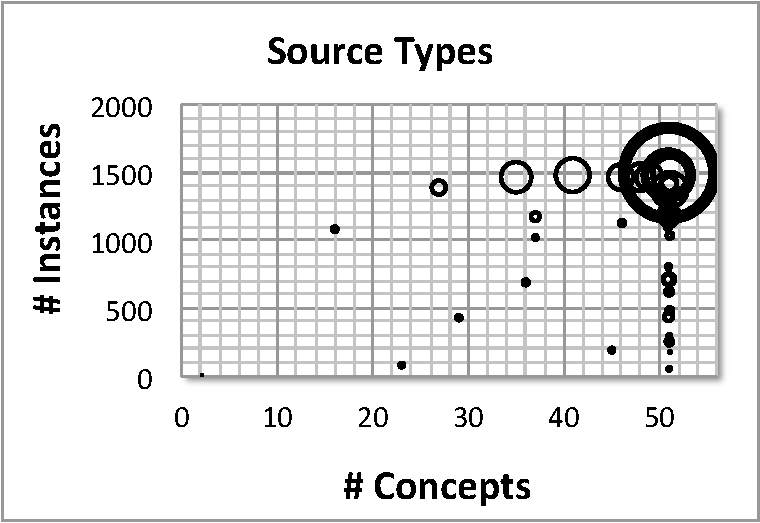
\includegraphics[clip,scale=0.4]{fig/sources.pdf}
	\caption{A fictional bubble chart describing the sources of a potential solution to a user query.}
	\label{fig:bubble}
	\end{center}
	\vspace{-10pt}
\end{figure}

We argue that first the query engine system should return a ranked list with {\em diverse} solutions on the Pareto frontier and mention the quality characteristics for the selected set of sources, the number of sources and the total integration cost. If the user selects to explore the content of the solution the system will present a bubble chart will all the sources in the solution. The dimensions of the bubble chart should be characterize the content of each source while the size of the bubble should correspond to the actual size (with respect to number of entries) of each source. We argue that the following dimensions are necessary to describe each source: (i) the {\em concept focus} of the source, i.e., number of different concepts mentioned in the source, and (ii) the {\em instance focus} of the source, i.e., the number of different instances mentioned in the source. If the user selects a specific bubble from the bubble chart details regarding the name and quality of the sources should be presented to the user. Notice that this information can be directly retrieved by the correspondence graph an does not need to be computed during query time. An example of such a bubble chart is shown in \Cref{fig:bubble}. Finally, we envision a system that will provide the user with the capability of exploring the neighborhood of a solution from the initial list. This can be done (i) either by removing sources from a running solution by allowing the user to select the ones to be removed from the bubble chart or (ii) by recommending solutions in the Pareto frontier neighborhood of the running solution. Notice that all the above functionalities require reasoning about the distance of solutions on the Pareto frontier introducing a new challenge.

%\ \\Descibe finding solutions on pareto frontier, describe how to diversify solutions. See papers on probing pareto frontier. 
%\ \\How to visualize solutions (coverage, freshness source bubble plot from SIGMOD 2014), how to explore the pareto frontier and neighborhood of solutions; a two level approach: {\bf Level 1:} return ranked list with ``distant" solutions on the pareto curve just mention quality characteristics, number of sources and cost. Present an average characteristic vector, no names or individual characteristics of sources, {\bf Level 2:} once the user selects a solution from the ranked list, then present bubble graph based on characteristics of sources. The two dimensions should be "concept focus" and "instance focus", bubble size should correspond to source size (whatever the source is reporting). The user can click to remove a source from the solution and the characteristics (overall quality, cost) of the solution should be updated. Apart from removing sources, neighboring solutions of the initial solution on the pareto frontier should be presented in a separate list. 


%\ \\Present architecture framework. Core module {\em knowledge graph and correspondence graph}. Modules:
%\begin{enumerate}
%\item Query engine: free-text queries mapped to entities and concepts. Quality metrics specified, cost specified, time-points of interest. 
%\item Correspondence graph: Go from entities to set of relevant sources (ground the domains of interest as a clusters of concepts and instances). 
%\item Source quality estimation: Given quality annotations of correspondence graph estimate the quality for future time points. The annotations will be either on edges from domain clusters to sources (for independent sources) or factor graphs at the cluster level for dependent sources. 
%\item Source selection module: Find source selection solutions on pareto frontier. Given quality and cost constraints find solutions on pareto frontier. 
%\item Query optimizer: find diverse solutions on pareto frontier. Speculative query answering for neighborhood on pareto frontier. 
%\item Result visualization: Present results to user. 
%\end{enumerate}

%\subsection{Supporting Diverse Integration Tasks}
%
%\ \\Analyze concepts of knowledge graph and correspondence graph. Describe construction of correspondence graph. How can you compute underlying quality characteristics of each source (i.e., compare content of sources).
%
%\subsection{Estimating the Quality of Integration}
%
%\ \\Describe how a correspondence graph can be extended with factor graphs and describe compilation techniques to compute quality of integration. Learn dependencies for different metrics. For each domain cluster: the domain corresponds to a union of concepts and instances.


\section{Related Work}
\label{sec:related}
Most of the prior work focuses on isolated aspects of data source management, and to our knowledge, there has been no systematic approach to developing a source management system over large numbers of data sources. There is much work on the problems of schema mapping and semantic integration of different
sources~\cite{cafarella:2009,venetis:11,oktie:11, oktie:13}. That line of work focuses on the construction of a global schema or a knowledge graph describing the domain of the data sources, and its final goal is not reasoning about the concepts that sources cover. Moreover, most of that work focuses on sources from a specific domain and does not present results for largely heterogeneous sources. Web table search~\cite{cafarella:2009,limaye:2010, dassarma:2012,yakout:2012, fan:2014} is also closely related to data source search. Most of the proposed techniques consider user queries and return tables related to specific keywords present in the query. However, the keyword based techniques fail to capture the semantics of the language, i.e., the intentions of the users, and thus they can only go as far as giving relevant hits. Using the knowledge graph as the entry point of data source search will enable us to clearly capture the intentions of the user and return more useful results. Further, extending data source search to recommend sets of sources to be integrated and analyzed collectively, as we propose to do, is a useful functionality in many domains (e.g., data driven journalism) where users are not experts and want an efficient way of exploring multiple data sources.  Finally, our work on source selection~\cite{dong:vldb13, rekatsinas:2014} has consider problems where all sources follow a common schema and focus on a single data universe.

\section{Conclusions}
\label{sec:conclusion}
In this paper, we argued that due to the vast amounts of available data sources it not beneficial for users to integrate all available sources as this can either be detrimental to the quality for the integration result or very expensive due to the fees sources charge to grant access to their data. We presented our vision for a data source management system that will enable users to not only discover the most valuable sources for their integration or analysis task given their budget but also enables the interactive exploration of different sets of sources allowing the user to truly understand the quality and cost trade-off between different integration options. We discussed the major challenges in building such a system including supporting fully heterogeneous integration tasks and multiple users, assessing the quality of data sources and enabling the interactive exploration over different sets of sources and presented a preliminary design of a source management system addressing these challenges. We believe that it is really about time for a new type of data portals that will allow data enthusiasts to find the most beneficial data sets for their tasks and limit the man-hours spent in validating the quality of data. 

\bibliographystyle{abbrv}
\bibliography{sourcify}
\end{document}
